\section{Putting it all together: water}

\subsection{}

\begin{frame}
  \frametitle{Putting it all together}
  \begin{center}
    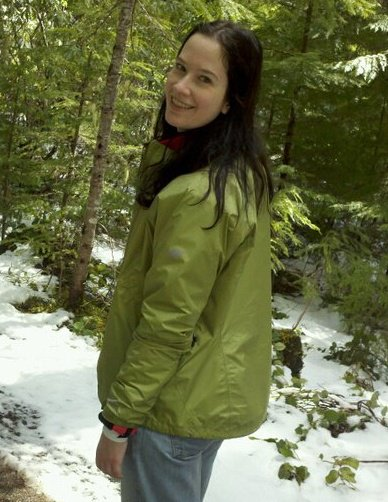
\includegraphics[height=3cm]{figs/HughesJessica}
    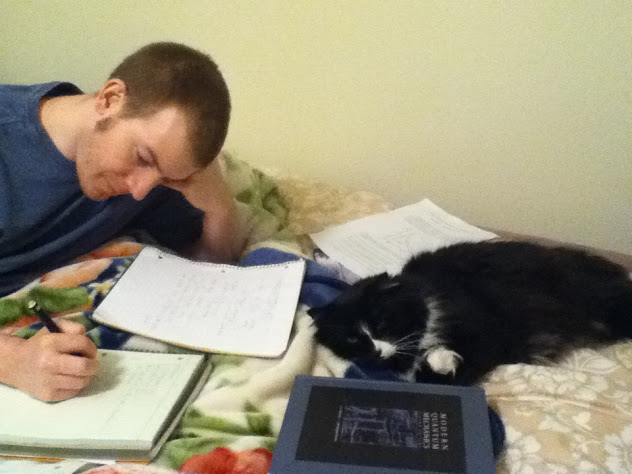
\includegraphics[height=3cm]{figs/KrebsEric}
  \end{center}
  \begin{block}{Statistical Associating Fluid Theory}
    \[
    F = F_{\textit{ideal gas}} + F_{\textit{hard spheres}} + F_{\textit{dispersion}} + F_{\textit{association}}
    \]
    We combine these terms to produce a classical density functional
    describing water.
  \end{block}
\end{frame}

\begin{frame}
  \frametitle{Homogeneous limit}
  \begin{center}
    \vspace{-1em}
    \includegraphics[height=6cm]{../../papers/water-saft/figs/pressure-with-isotherms-truncated}
   \end{center}
  Five SAFT empirical parameters taken from\\\hfill Clark \emph{et al.}, \emph{Mol. Phys.}
  (2006)
\end{frame}

\begin{frame}
  \frametitle{Homogeneous limit}
  \begin{center}
    \vspace{-1em}
    \includegraphics[height=7cm]{../../papers/water-saft/figs/surface-tension}
  \end{center}
  \vspace{-1.5em}
  One additional empirical parameter (in dispersion) used to fit
  surface tension.
\end{frame}

%% \begin{frame}
%%   \frametitle{Two hard rods}
%%   \begin{center}
%%     \vspace{-1em}
%%     \includegraphics[height=8cm]{figs/density-rods-in-water}
%%   \end{center}
%%   \vspace{-1.5em}
%% \end{frame}

\begin{frame}
  \frametitle{Hydration of a hard sphere}
  \begin{center}
    \vspace{-1em}
    \includegraphics[height=7cm]{figs/sphere-energy}
  \end{center}
  \vspace{-1.5em}
\end{frame}

\begin{frame}
  \frametitle{Conclusion \#2}
  \vspace{2em}
  \begin{block}{Hard sphere contact}
    \vspace{-6em}
    \hfill
    \includegraphics[height=2cm]{figs/walls-10}
    \includegraphics[height=2cm]{figs/walls-40}
    \begin{itemize}
    \item Found and tested an accurate functional for the correlation
      function at contact for hard spheres
    \item Reasonably efficient: scales like the hard sphere free
      energy
    \end{itemize}
  \end{block}
  \begin{block}{Water}
    \begin{itemize}
    \item Developed and tested a SAFT-based functional for water
    \end{itemize}
  \end{block}
  \begin{block}{Future work}
    \begin{columns}
      \begin{column}{0.7\columnwidth}
        \begin{itemize}
        \item Test dispersion versus MC
        \item Renormalization group for critical point
        \item Hard polyhedra for directional correlation
        \end{itemize}
      \end{column}
      \begin{column}{0.5\columnwidth}
        \begin{itemize}
        \item Dielectric interactions
        \item Softening the spheres
        \item Coupling with solute
        \end{itemize}
      \end{column}
    \end{columns}
  \end{block}
\end{frame}
